%	DOCUMENT TYPE
\documentclass[notitlepage,11pt,nofootinbib]{revtex4-1}
% \documentclass[aps,prb,notitlepage,11pt,nofootnoteinbib]{revtex4-1}
% \documentclass[aps,preprint,prb,linenumbers]{revtex4-1}

%	PACKAGES
\usepackage[utf8]{inputenc}
\usepackage{amssymb,amsmath,amsfonts,mathtools,dsfont,bm,enumitem}
\usepackage[usenames,dvipsnames]{xcolor}
\usepackage[pdftex]{graphicx}
\usepackage[pdftex,plainpages=false,colorlinks=true,linkcolor=Red, citecolor=blue, urlcolor=blue]{hyperref}
\usepackage[most]{tcolorbox}
\usepackage{empheq}
\usepackage{listings}
\lstset{language=python}

%	FONT & CUSTOM SYMBOLS
%\usepackage{esint}
%\usepackage[T1]{fontenc}
%\usepackage{microtype}
% \usepackage[fullfamily,lf,minionint,openg,loosequotes]{MinionPro}
% \usepackage{libertine}
% \usepackage{txfonts}

%%%% vector (bold)
% \renewcommand{\vec}[1]{\bm{\mathrm{#1}}}
\renewcommand{\vec}[1]{\bm{#1}}

%%%% tensor
% \usepackage{stackengine}\stackMath
% \def\lvec{{\rotatebox{180}{$\mkern+0mu\mathchar"017E$}}}
% \def\tensign{\smash{\stackon[-1.99pt]{\mkern-4mu\mathchar"017E}{\rotatebox{180}{$\mkern+0mu\mathchar"017E$}}}}
% \def\tensor#1{\def\useanchorwidth{T}\stackon[-4.3pt]{#1}{\,\tensign}}


%	DOCUMENT
\begin{document}

\title{\bf Temperature-agnostic analytic continuation of conductivity\\demonstrated with neural networks}
\author{S. \surname{Verret}}
\affiliation{Institute for Learning Algorithms (MILA), Montr\'eal, Canada}
\affiliation{Institut Quantique (IQ), Sherbrooke, Canada}
\date{\today}
% \keywords{}

\begin{abstract}

\end{abstract}

\maketitle
\vspace{-.5cm}
\tableofcontents

\section{Temperature-agnostic analytic continuation}

\subsection{Analytic continuation of conductivity}

The starting point of this report is the following relation (partly derived in appendix) between the Matsubara response function $\Pi(i\omega_n)$ and the optical conductivity $\sigma(\omega)$,
\begin{align}
\Pi(i\omega_n) 
=
\int_{-\infty}^{\infty} \frac{d\omega}{\pi} \frac{\omega^2}{\omega^2+\omega_n^2}
\text{Re}\{ \sigma(\omega) \}.
\label{Pi_continuation}
\end{align}
Here, $\omega$ is a frequency or energy (we set $\hbar=1$), $\omega_n=2\pi k_BTn$ are Matsubara frequency, $T$ is the temperature, and $k_B$ is the Boltzmann constant.
Four our purpose, the term ``analytic continuation'' refers to the problem of inverting equation~\eqref{Pi_continuation}. That is, recover a numerical estimate of $\text{Re}\{ \sigma(\omega) \}$ given a numerical estimate for $\Pi(i\omega_n)$.


Two special cases of the above equation will be of particular importance. First, the value $\Pi(i\omega_n=0)$ which corresponds to the normalization of $\text{Re}\{ \sigma(\omega) \}$,
\begin{align}
\Pi(0) 
=
\int_{-\infty}^{\infty} \frac{d\omega}{\pi}
\text{Re}\{ \sigma(\omega) \}.
\label{Pi_normalization}
\end{align}
Second, values of $\Pi(i\omega_n)$ at high $\omega_n$ and values of $\text{Re}\{ \sigma(\omega) \}$ at high $\omega$ (the tails) are related by
\begin{align}
\lim_{\omega_n\rightarrow\infty}
\omega_n^2
\Pi(i\omega_n)
=
\int_{-\infty}^{\infty} \frac{d\omega}{\pi}\omega^2 
\text{Re}\{ \sigma(\omega) \}.
\label{Pi_moment}
\end{align}

\subsection{Dimensionless formulation}
\label{sec_dimensionless}
We can obtain a dimensionless version of~\eqref{Pi_continuation} by dividing it by~\eqref{Pi_normalization}. To clarify the dimensional analysis,we substitute $\omega_n = 2\pi k_BTn$, and temporarily restore $\hbar$,
\begin{align}
\frac{\Pi(i\omega_n)}{\Pi(0)}
&=
\int_{-\infty}^{\infty} d\omega \frac{\omega^2}{
\omega^2+
\big(\frac{2\pi k_B}{\hbar}T\big)
^2n^2
}\left(
\frac{\text{Re}\{ \sigma(\omega) \}}
{\int_{-\infty}^{\infty} d\omega \text{Re}\{ \sigma(\omega) \}}
\right).
\label{dimensionless}
\end{align}
We will denote the left-hand side as a vector $\vec \Pi$, \begin{align}
\Pi_n = \frac{\Pi(i\omega_n)}{\Pi(0)} 
% = \frac{\Pi(i2\pi k_B T n)}{\Pi(0)},
\end{align}
and the term in parenthesis as a density function $p(\omega)$,
\begin{align}
p(\omega) =
\frac{\text{Re}\{ \sigma(\omega) \}}
{\int_{-\infty}^{\infty} d\omega \text{Re}\{ \sigma(\omega) \}}.
\label{eq_def_density}
\end{align}
These are natural dimensionless input $\vec\Pi$ and output $p(\omega)$ for the analytic continuation problem. We then rewrite \eqref{dimensionless} with a change of variable $\omega\rightarrow s\omega$
\begin{align}
\Pi_n
&=
\int_{-\infty}^{\infty} d\omega \frac{\omega^2}{\omega^2 + \left(\frac{2\pi k_B}{\hbar}T\right)^2n^2}
p(\omega),
\label{dimensionless_with_p1}
\\
&=
\int_{-\infty}^{\infty} d\omega \frac{\omega^2}{\omega^2 + \left(\frac{2\pi k_B}{\hbar}\frac{T}{s}\right)^2n^2}
sp(s\omega),
\label{dimensionless_with_p2}
\end{align}
which lets us isolate an alternative integrand argument $sp(s\omega)$, where $s$ fits the definition of a \emph{scale parameter}.
If we consider that $s$ carries the units of frequency, $\omega$ becomes a dimensionles continuous variable (analogous to the integer $n$ in matsubara frequencies) and the term $\frac{2\pi k_B}{\hbar}\frac{T}{s}$ then corresponds to a dimensionless temperature.

\subsection{Temperature-agnostic formulations}
\label{section_temperature_agnostic}
The above dimensionless formulation shows that there is a degenerancy between analytic continuation problems at different temperatures. We can make this degenerancy explicit by writing integral~\eqref{dimensionless_with_p1} as a functional $\Pi_n = \Pi_n[p(\omega)](T)$, such that lines~\eqref{dimensionless_with_p1} and~\eqref{dimensionless_with_p2} become 
\begin{align}
\Pi_n[p(\omega)](T) = \Pi_n[sp(s\omega)](T/s).
\label{degenerancy}
\end{align}
This equality tells us that the same response function components $\Pi_n$ can be found at different temperatures $T$ and $T/s$ for respective distributions $p(\omega)$ and $sp(s\omega)$. In other words, the input $\vec \Pi$ has a continuum of compatible output $sp(s\omega)$, since $s$ can take any value. Thus, without the temperature $T$ or the frequency scale $s$ specified, the analytic continuation task is ambiguous. For a well defined problem, we must either fix $T$ or $s$.

\paragraph*{Fixing $T$}
Working from a single temperature $T_\text{{ref}}$ and considering $s=T_\text{{ref}}/T$ in~\eqref{degenerancy}
\begin{align}
    \Pi_n[p(\omega)](T_\text{{ref}}) = \Pi_n[\tfrac{T_{\text{ref}}}{T} p(\tfrac{T_{\text{ref}}}{T}\omega)](T),
    \label{eq_fix_T}
\end{align}
we see that results at any $T$ can be obtained by rescaling the distribution $p(\omega)$ obtained at~$T_\text{{ref}}$. This is the first way to get temperature-agnostic analytic continuation.

\paragraph*{Fixing $s$}
Working with a single $s$ is also possible, but requires more care. However, as we will argue in the rest of this report, fixing $s$ provides several desirable advantages over the simpler fixed-$T$ approach. In the fixed-$s$ approach, we redefine analytic continuation as the task mapping all response function vectors $\Pi_n = \Pi_n[sp(s\omega)](T/s)$ (obtained at temperature $T/s$ and density function $sp(s\omega)$ for any~$s$) to a single \emph{reference} density $p(\omega)$ (independent of $s$):
\begin{align}
    \Pi_n[sp(s\omega)](T/s) &\longrightarrow p(\omega) &\text{for any }s.
    \label{eq_agnostic_ac}
\end{align}
With analytic continuation defined this way, we can ignore temperature alltogether and work in terms of $\vec \Pi$ and $p(\omega)$ only. This is the second way to get temperature-agnostic analytic continuation.

However, two things must be clarified for the fixed-$s$ scheme to be well-defined. First, we must choose the reference $p(\omega)$ to represent all other $sp(s\omega)$. Second,
we must explain how to recover the missing scale $s$ from $\vec \Pi$ alone once the reference $p(\omega)$ is obtained. These considerations are respectively adressed in the next two sections.

\subsection{Fixing the second moment}
\label{sec_data_rescaling}
Suppose we want to train a neural network $p_{\vec \theta}(\omega, \vec \Pi)$ to perform the analytic continuation task defined in~\eqref{eq_agnostic_ac}. Training such neural networks requires training data, more specifically several thousand pairs of inputs $\vec \Pi$ and output targets $p(\omega)$. Here we explain how to remove any $sp(s\omega)$ from the training dataset to get only reference distributions $p(\omega)$.

To create each ($\vec \Pi$, $p(\omega)$) pair, we start by generating an arbitrary distribution $p_0(\omega)$. We will describe a way to do so in section~\ref{sec_distribution}. For now, let us simply presume the latter is not a reference distribution; it is inherently scaled as $p_0(\omega)=sp(s\omega)$, for some unknown $s$.
To find $s$, we make a choic: we define all reference $p(\omega)$ so that they have the same second central moment $\mu_2$. This $\mu_2$ becomes a constant of the dataset,
\begin{align}
\mu_2
&=
\int d\omega \omega^2 p(\omega).
\label{eq_sec_moment}
\end{align}
Performing the change of variable $\omega \rightarrow s\omega$ in~\eqref{eq_sec_moment}, we get
\begin{align}
\mu_2&=
s^2 \int d\omega \omega^2 p_0(\omega),
\end{align}
from which we isolate $1/s$ as
\begin{align}
\frac{1}{s}
&=
\sqrt{
\frac{1}{\mu_2}
\int d\omega \omega^2 p_0(\omega),
}
\end{align}
letting us prepare the reference $p(\omega)$ from $p_0(\omega)$ as
\begin{align}
p(\omega) 
&=
\frac{1}{s}p_0\big(\frac{1}{s}\omega\big).
\end{align}
Preparing every conductivity like this produces a dataset with only reference $p(\omega)$ as targets.

Fixing $\mu_2$ have three noteworthy advantages. First, all reference distributions will have similar widths in the $\omega$ space; there will be no exessively narrow or wide $p(\omega)$, this is useful when working on a frequency grid. 
Second, if the generation process for $p_0(\omega)$ allows one to control the second central moment of the distribution analytically, the correct scale can be enforced without numerical overhead (we did not take advantage of this in the current work).
And third, the constant $\mu_2$ simplifies the recovery of conductivity explained in the next section.

% Note that constant second moment $\mu_2 = \mathbb E[\omega^2]$ is not the only possibility. One could also prepare $p(\omega)$ with constant $\mathbb E [\omega^4 - \mathbb E[\omega^2]^2]$, for example.
% The latter notably provides stronger guarantees on the domain of $p(\omega)$, which can be shown using a variant of Chebyshev's inequality. However, if one is to use the high frequency information from $\Pi(i\omega_n)$ to extract the real frequency scale, then using the second moment is required.



\subsection{Recovering conductivity}
\label{sec_usage}
Suppose we have access to a neural network $p_{\vec\theta}(\omega,\vec\Pi)$ (with $\vec \theta$ denoting all adjustable parameters) which takes $\vec \Pi$ as an input and approximates a single reference $p(\omega)$ as an output,
\begin{align}
p_{\vec\theta}(\omega,\vec \Pi)\approx p(\omega).
\end{align}
To perform analytic continuation, a user starts from a response function $\Pi(i\omega_n)$ and prepare the according dimensionless input vector $\vec \Pi$, with
\begin{align}
\Pi_n = \frac{\Pi(i\omega_n)}{\Pi(0)}.
\end{align}
Using the latter as an input for the algorithm, the user obtains the reference $p_{\vec\theta}(\omega,\vec \Pi)\approx p(\omega)$. However, the user desires not the reference distribution $p(\omega)$, but one of the many possible $sp(s\omega)$ corresponding to their particular temperature. 
From the change of variable $s\omega\rightarrow \omega$ in~\eqref{Pi_moment},
\begin{align}
    \lim_{\omega_n\rightarrow\infty}\omega_n^2
    \frac{\Pi(i\omega_n)}{\Pi(0)}
    &=
    \int_{-\infty}^{\infty}d\omega \omega^2 sp(s\omega)
    \\
    &=
\frac{1}{s^2}
\int\limits_{-\infty}^{\infty}d\omega \omega^2 p(\omega)
\\
&= \frac{\mu_2}{s^2},
\end{align}
$s$ can be isolated as 
\begin{align}
s
&=
\sqrt{
    \frac{1}{\mu_2}
    \lim\limits_{\omega_n\rightarrow\infty}\omega_n^2
    \dfrac{\Pi(i\omega_n)}{\Pi(0)}
    }.
    \label{user_s}
\end{align}
This expression depends on the user's temperature through $\omega_n = 2\pi n k_B T$. 
The user can then recover the desired conductivity by combining this $s$ with~\eqref{Pi_normalization} and~\eqref{eq_def_density},
\begin{align}
\text{Re}\{ \sigma(\omega) \} = \pi\Pi(0) 
s p_{\vec \theta}(s\omega, \vec \Pi).
\end{align}



\section{Using neural networks}

\subsection{Discrete formulation}
\label{section_discrete}

Analytic continuation with neural networks is typically done with vector-to-vector neural networks~\cite{Fournier2020,Xie2019,Yoon2018,Kades2019}. The output of the neural network is then a vector $\hat{\vec p} = p_{\vec \theta}(\vec \Pi)$ which targets the desired function $p(\omega)$ on a grid of real frequencies,
\begin{align}
\omega_m &=
\Delta\omega m.
&\text{with }m\in\{-M,...1,0,1,...,M\}.
\label{eq_discrete_grid}
\end{align}
the spacing between frequencies $\Delta \omega$ can also be expressed as $\Delta\omega =\omega_{\text{max}}/M$ with $\omega_{\text{max}}$ marking the end of the sampling. Discretizing~\eqref{dimensionless_with_p1} on this grid,\begin{align}
[\vec \Pi]_n
&\approx
\sum_{m}
\Delta\omega \frac{\omega_m^2}{\omega_m^2+\omega_n^2} p(\omega_m)
\label{discretized_continuation_1}
\\
&\approx
\sum_{m}
\frac{m^2}{m^2+(\frac{2\pi k_B}{\hbar}\frac{T}{\Delta\omega}n)^2} \Delta\omega p(\Delta\omega m)
\\
&\approx
\sum_{m}
\frac{m^2}{m^2+(\frac{2\pi k_B}{\hbar}\frac{T}{\Delta\omega}n)^2} 
[\vec p]_m
\label{discretized_continuation}
\end{align}
we define the target vector $\vec p$ as
\begin{align}
    [\vec p]_m = \Delta\omega p(\Delta\omega m).
\end{align}
Training the neural network then amounts to minimize the expected distance between $\hat{\vec p}$ and $\vec p$ over a large training set of $(\vec \Pi,\vec p)$ pairs (see section~\ref{sec_training}).

One must be careful and remember that discretizing integrals as above is only an approximation. 
As such, we recommend to avoid sums like~\eqref{discretized_continuation} and perform more accurate integration of $p(\omega)$ whenever possible.
In fact, seeing the kernel in~\eqref{discretized_continuation} as a matrix and inverting that matrix is not the same as solving the continuous inversion problem. This can be understood by imagining the limiting case in which one uses only a handful of points to approximate the integral. There is additional difficulty due to the discretization in the matrix problem, but it is not intrinsic to the continuous problem. Equating the two can be misleading.

Note that $\Delta\omega$ occupies the same position as the scale parameter $s$ which was the focus of the previous section, and indeed, it will play precisely this role in what follows.

\subsection{Normalization}
\label{sec_normalization}
For various reasons (see section~\ref{sec_training}), it is beneficial to make the neural network's output components $p_m$ sum to one. Considering the discretized normalization integral for $p(\omega)$,
\begin{align}
\int d\omega p(\omega) = 1 \approx \sum_m \Delta\omega p(\Delta\omega m),
\end{align}
we see that $p_m$ must correspond to $[\vec p]_m = \Delta\omega p(\Delta\omega m)$, as defined in the previous section.
There is no problem in combining the rescaling $p(\omega)\rightarrow sp_0(s\omega)$ discussed in sections~\ref{sec_dimensionless},~\ref{section_temperature_agnostic} and~\ref{sec_data_rescaling} with the above normalization. We will note it $\vec p \rightarrow \vec p_s$.
\begin{align}
    [\vec p_s]_m = s\Delta\omega p_0(s\Delta\omega m).
\end{align}
Both $\vec p$ and $\vec p_s$ sum to one, because both $p(s)$ and $sp(s\omega)$ integrate to one. Note, however, that the $\omega_m$ values at which those functions are sampled are not the same; respectively $\Delta\omega m$ and $s\Delta\omega m$.


\subsection{Preparing data}

Training the neural network requires to prepare a dataset. This section enumerate four approaches to do so, and discuss them. In all cases, the idea is to generate a large number of random normalized functions $p_0(\omega)$ and use each of them to obtain one input-target pair, ($\vec \Pi$, $\vec p$).

\paragraph*{Fixing $T$}
The simplest way is to work at fixed temperature.
\begin{enumerate}
    \item \label{fixT}
    \begin{itemize}
        \item[$\vec p$:] Sample $p_0(\omega)$ on the frequency grid $\omega_m=\Delta\omega m$ and normalize, $[\vec p]_m = \Delta\omega p_0(\Delta\omega m)$.
        \item[$\vec \Pi$:] Using $p_0(\omega)$, integrate~\eqref{dimensionless_with_p1} numerically, at chosen temperature $T_{\text{ref}}$.
    \end{itemize}
\end{enumerate}
Note that generating $(\vec\Pi, p_0(\omega))$-pairs at fixed temperature naturally produce multiple scales~$s$. By this, we mean that multiple $p_0(\omega)=sp(s\omega)$ from the dataset could share the same reference $p(\omega)$ but with different values of~$s$.
Thus, using a single temperature $T_{\text{ref}}$ to generate a dataset is sufficient to cover multiple dimensionless temperature $\mathcal T\propto\frac{T}{s}$. This is why the fixed $T_{\text{ref}}$ scheme can be used to get results at other temperatures as explained in section~\ref{section_temperature_agnostic}. However, we will see below that working this way introduces spurious correlations in the dataset.

\paragraph*{Fixing $s$}
As we'll see, working at fixed scale $s$ provides more control over the correlations in the dataset. There are two equivalent ways to proceed.
\begin{enumerate}[resume]
\item \label{rescaled}
\begin{itemize}
    \item[$\vec p$:] Get the reference distribution $p(\omega) = \tfrac{1}{s}p_0(\tfrac{1}{s}\omega)$ as explained in section~\ref{sec_data_rescaling}. Sample it with the frequency grid $\omega_m=\Delta\omega m$, and normalize, $[\vec p]_m = \frac{1}{s}\Delta\omega p_0(\frac{1}{s}\Delta\omega m)$.
    \item[$\vec \Pi$:] Using the rescaled $p(\omega)$, integrate~\eqref{dimensionless_with_p1} numerically at any desired temperature $T$.
\end{itemize}
\item \label{p0rescaled}
\begin{itemize}
    \item[$\vec p$:] Sample the original distribution $p_0(\omega)$ on a new frequency grid $\omega_m=\frac{\Delta\omega}{s} m$ with $\frac{1}{s}$~obtained as described in section~\ref{sec_data_rescaling} and normalize, $[\vec p]_m = \frac{1}{s}\Delta\omega p_0(\frac{1}{s}\Delta\omega m)$.

    \item[$\vec \Pi$:] Using the original distribution $p_0(\omega)$, integrate~\eqref{dimensionless_with_p1} at any desired temperature $T/s$.
\end{itemize}
\end{enumerate}
Approaches \ref{rescaled} and \ref{p0rescaled} yield the same $\vec p$ and $\vec \Pi$ because of the degenerancy covered in section~\ref{section_temperature_agnostic}. Namely, approach~\ref{rescaled} uses the distribution $p(\omega)$ at temperature $T$ whereas approach~\ref{p0rescaled} uses the distribution $p_0(\omega)=sp(s\omega)$ at temperature $T/s$. Note that the sampling grid must match the scale $s$ to obtain the same $\vec p$ out of $p(\omega)$ and $p_0(\omega)=sp(s\omega)$.

\paragraph*{Spurious correlations}
Let us now explain why approaches \ref{rescaled} and \ref{p0rescaled} provide more control. We consider a fourth way of generating data in which we use the rescaled target $\vec p$ but fixed $T_{\text{ref}}$ input $\vec \Pi$, as in ~\ref{fixT}.
\begin{enumerate}[resume]
    \item \label{spurious}
    \begin{itemize}
        \item[$\vec p$:] Sample the original distribution $p_0(\omega)$ on a new frequency grid $\omega_m=\frac{\Delta\omega}{s} m$ with $\frac{1}{s}$~obtained as described in section~\ref{sec_data_rescaling} and normalize $[\vec p]_m = \frac{1}{s}\Delta\omega p_0(\frac{1}{s}\Delta\omega m)$.

        \item[$\vec \Pi$:] Using the original distribution $p_0(\omega)$, Integrate~\eqref{dimensionless_with_p1} at temperature $T_{\text{ref}}$.
    \end{itemize}
\end{enumerate}
Because of the fixed $T_{\text{ref}}$, approaches~\ref{fixT} and~\ref{spurious} both lead to spurious correlations. Indeed, when all $\vec \Pi$ are computed at the same temperature, a narrow distribution $p_0(\omega)$ leads to a fast-decreasing $\vec \Pi$, and a wide $p_0(\omega)$ leads to slow-decreasing $\vec \Pi$, as expected from the tail relation~\eqref{Pi_moment}.
In approach~\ref{fixT}, this correlation should manifest directly: fast-decreasing $\vec \Pi$ are paired with narrow $\vec p$ (meaning only the first few components of $\vec p$ are non-negligible) while slow-decreasing $\vec \Pi$ are paired with wide $\vec p$ (most components being non-negligible). This is what we mean by ``spurious correlation'' in that case.
In approach~\ref{spurious}, the spurious correlations get more subtle. Since targets~$\vec p$ are rescaled to the same width (the rescaling leads to fixed second moment), the correlations between the width of $\vec p$ and decreasing rate of $\vec \Pi$ is removed. However, other spurious correlations might remain depending on the process used to generate $p_0(\omega)$. For example, if this process led to simpler structure (fewer peaks) for narrow $p_0(\omega)$, and more complex structure (many peaks) for wide $p_0(\omega)$ (as in section~\ref{sec_distribution}), then the these correlations between the structure of $p_0(\omega)$ and its width gets transferred through the one between the width of $p_0(\omega)$ and the decreasing rate of $\vec \Pi$. As a result, fast-decreasing $\vec \Pi$ are paired with simpler-structured $\vec p$ and slow-decreasing $\vec \Pi$ are paired with more complex-structured $\vec p$. This is what we mean by ``spurious correlation'' in that case.
Such spurious correlations may or may not be desirable, but one must be aware they exists.

Approaches~\ref{rescaled} and~\ref{p0rescaled} completely avoid these uncontrolled correlations between the decrease of $\vec \Pi$ and the width or structure of $\vec p$. Approach~\ref{rescaled} do so by rescaling $p_0(\omega)$ and working only with the new function $p(\omega)$ which has fixed width (fixed second moment), and approach~\ref{p0rescaled}, which is equivalent, instead adjusts the temperature $T/s$ and the frequency grid to the second moment of $p_0(\omega)$.
With these approaches, if a single value of $T$ is used, all $\vec \Pi$ end up with the same decrease rate (because all $\vec p(\omega)$ have the same width). In order to get a dataset which cover multiple dimensionless temperature $\mathcal T\propto\frac{T}{s}$, randomly sampled values of $T$ must be used. One can then control spurious correlations, if desired, by varying $T$ as a function of $p_0(\omega)$.

The above considerations clarify the kind of bias which is induced when preparing the dataset. Constraining the output space of analytic continuation by choosing the training domain is the main benefit of using machine-learning for analytic continuation~\cite{Arsenault2017}. This bias in the space of allowed $p(\omega)$ is desirable since it acts as a form of regularization. Similarly, a bias in the way this space changes with temperature (the spurious correlations discussed above) might also be desirable. Indeed, high temperature $\vec \Pi$ don't provide as much information as low temperature $\vec \Pi$ and therefore simpler $p(\omega)$ might be easier to learn at high temperatures. As we just described, by being careful with the dataset generation, it is possible to control these biases.

\subsection{Training details}
\label{sec_training}

\paragraph*{Neural network} We considered the case where the input and output sizes are respectively $N=128$ and $M=512$. The optimal neural network we found is fully connected, with four hidden layers roughly of dimension $1000$, $1350$, $1700$, and $1700$. We use rectified linear unit (ReLU) activation functions and a Softmax output unit (producing a normalized $\vec p$). The Softmax requires normalized target outputs as explained in section~\ref{sec_normalization}. Weights are initialized using Xavier initialization.

\paragraph*{Standardized inputs} Any data that enters the neural network is standardized as $(\vec \Pi - \vec\mu)/\vec\sigma$, where $\vec \mu = \mathbb{E}[\vec \Pi]$ and $\vec \sigma = \sqrt{\mathbb{E}[\vec \Pi^2] - \mathbb{E}[\vec \Pi]^2}$ are respectively the average and the standard deviation of the training inputs dataset(element-wise), with expectation values taken over the training set only. The random noise added to $\vec \Pi$ to simulate Quantum Monte-Carlo response functions is renewed at every epoch and it is added before standardization.

\paragraph*{Loss functions} As a training objective, we compared the performance of cross-entropy, 
\begin{align}
    \text{CE}(\vec p,\hat{\vec p}) = \frac{1}{M}\sum_m p_m \log \hat{p}_m
\end{align}
mean-square error, 
\begin{align}
    \text{MSE}(\vec p,\hat{\vec p}) = \frac{1}{M}\sum_m \sqrt{(p_m - \hat{p}_m)^2}
\end{align}
and mean-absolute error
\begin{align}
    \text{MAE}(\vec p,\hat{\vec p}) = \frac{1}{M}\sum_m |p_m - \hat{p}_m|.
\end{align}
We found that using the mean-absolute error as the training objective leads to better final performance for all three losses.

\paragraph*{Optimizer} We use the Adam optimizer with learning rate of $\alpha = 8\times10^{-5}$ and a scheduler decreasing the rate as $\alpha \rightarrow 0.216\alpha$ whenever the validation loss doesn't improve for five straight epochs. That decrase stops when the learning rate reach $\alpha\sim10^{-10}$. We also use learning rate warm-up, linearly increasing $\alpha$ from zero to its value of $\alpha = 8\times10^{-5}$ during the first epoch.

\paragraph*{Regularization} Our random search for optimal hyper-parameters revealed that neither L2 regularization, dropout, nor batchnorm improve results. However, using slightly larger input noise at training time than at test time leads to better performance, and training on more complex data (Beta peaks) can lead to better performance on simple data (Gaussian peaks) than training on simple data.

\subsection{Usage details (inference)}

Once the user obtain the estimate $\hat{\vec p}$ with the neural network, the only thing left to do is to find the frequency grid $\Delta\omega$ on which to interpret that estimate. Considering the discretization~\eqref{discretized_continuation_1} for the special case of the tail relation~\eqref{Pi_moment},
\begin{align}
    2\pi k_B T \lim_{n\rightarrow \infty}n^2 \Pi_n = \Delta\omega^2 \sum_m m^2 p_m
\end{align}
We see that $\vec \Pi$ and $\vec p$ provide a closed relation between the temperature and the frequency spacing. If we assume that the discretization is a good approximation for the integral and that the last component $\Pi_N$ correctly captures the limit $n\rightarrow\infty$, then we can cast this relation as
\begin{align}
    \Delta\omega^2 = 
    \frac{
        2\pi k_B 
        % \lim_{n\rightarrow \infty}n^2 \Pi_n
        N^2 \Pi_N
    }{
        \sum_m m^2 p_m
    }
    T.
\label{eq_minimal_user}
\end{align}
This is a discrete version of~\eqref{user_s} which can be used to recover $\Delta\omega$ from the user's temperature $T$. In principle, however, the continuous version should be preferred. In particular, a simple way to improve on~\eqref{eq_minimal_user} is to use a better estimate for $\lim_{\omega_n\rightarrow \infty}\omega_n^2 \Pi_n$, than $2\pi k_B T N^2\Pi_N$. Note that if the fixed $T_{\text{ref}}$, this task is considerably simplified, as one can use $T/T_{\text{ref}}$

\section{Generating density functions}
\label{sec_distribution}
\subsection{Gaussian peaks}
The first way to generate random distributions is a weighted sum of Gaussian peaks 
\begin{align}
p(\omega)
=
\sum_{j=1}^{N} 
\frac{\pi A_j}{\sqrt{2\pi} \sigma_j}
\exp\bigg(-\frac{1}{2}\Big(\frac{\omega-\omega_j}{\sigma_j}\Big)^2\bigg).
\end{align}
Each peak parametrized by weight $A_j$, center $\omega_j$, and width $\sigma_j$.

Most machine learning papers on analytic continuation were trained on sets of Gaussian peaks as described above~\cite{Arsenault2017, Yoon2018, Xie2019, Fournier2020}. The most influential paper in that respect is arguably that of Arsenault et al~\cite{Arsenault2017}, which correctly identifies the importance of the data as a mean for regulation. Unfortunately, some of the constraints used for their data generation are described qualitatively, which prevents faithful reproduction. The work of Yoon et al.~\cite{Yoon2018} uses a somewhat complicated and arbitrary distribution for the number of peaks. The dataset defined by Fournier et al.\cite{Fournier2020} and re-used in Xie et al.\cite{Xie2019}, are more straigthforward to generate. Note however, that their definition implies that $A_j=\sigma_j$ which favours very rounded distributions.


\subsection{Beta peaks}
The second way to generate random distributions is a weigthed sum of $\beta$-peaks
\begin{align}
p(\omega)
=
\sum_{j=1}^{N} 
\frac{\pi A_j}{\tilde{\sigma}_j}
\text{Beta}\bigg(
\frac{\omega-\tilde{\omega}_j}{\tilde{\sigma}_j}
;\alpha_j,\beta_j
\bigg).
\end{align}
Each peak is parametrized by the amplitude $A_j$, the $\alpha_j$ and $\beta_j$ of the Beta distribution,
\begin{align}
\text{Beta}(x;\alpha,\beta) 
&=
\frac{\Gamma(\alpha+\beta)}{\Gamma(\alpha)\Gamma(\beta)} x^{1-\alpha}(1-x)^{1-\beta},
\end{align}
and, since the latter is only non-zero for $0\leq x\leq 1$, the center $\omega_j$ and the width $\sigma_j$ of the peaks we generate must be adjusted to the mean and standard deviation of the distribution, as
\begin{align}
\tilde{\omega}_j
&=
\omega_j+\sigma_j
\frac{\alpha_j}{\alpha_j+\beta_j}
\\
\tilde{\sigma}_j
&=
\sigma_j
\bigg(
\frac
{(\alpha_j+\beta_j+1)(\alpha_j+\beta_j)^2}
{\alpha_j\beta_j}
\bigg)^{\frac{1}{2}}.
\end{align}

Note that for large $\alpha=\beta$, the Beta distribution becomes very similar to the Gaussian distribution. Values of $\alpha=\beta\gtrsim 10$ are sufficient to make them indistinguishable on a plot. However, the tails of the Gaussian extend to infinity, whereas the tails of the Beta distribution are always bounded within $0 \leq \frac{\omega-\tilde{\omega}_j}{\tilde{\sigma}_j} \geq 1$. Nevertheless, we hypothesize that learning with Beta-distribution will easily generalize to Gaussian distributions.

Note also that for disctrete values of $\alpha$ and $\beta$, the beta distribution is identical to Bernstein polynomials
\begin{align}
b_{m,n}(x)
&=
\binom{m}{n} x^n(1-x)^{m-n}
\end{align}
where $\binom{m}{n}$ is the binomial coefficient, and $m$ and $n$ are integer parameters. They can be related to the real-valued $\alpha$ and $\beta$ of the Beta distribution by
\begin{align}
m &= \alpha+\beta-2
\\
n &= \alpha-1.
\end{align}
The normalization, mean, and standard deviation of these polynomials are respectively given by
\begin{align}
a_{m,n}
&=
\frac{1}{m+1},
\\
\mu_{m,n}
&=
\frac{1+n}{2+m},
\\
\sigma_{m,n}
&=
\bigg(
\frac{(1+n)(2+n)}{(2+m)(3+m)}
-
\frac{(1+n)^2}{(2+m)^2}
\bigg)^{\frac{1}{2}}.
\end{align}
so it is possible to adjust them to control their center and width as we did for the Beta distribution. It is worth noting that Bernstein polynomials are used to write Bezier curves in polynomial form, and they provide a constructive proof of the Weierstrass approximation theorem.



\begin{acknowledgments}
This project was started in close collaboration with Reza Nourafkan and André-Marie Tremblay. I must also acknowledge additional useful discussions with Yoshua Bengio, Maxime Charlebois, Samuel Desrosiers, Sébastien Lachapelle, Vincent Mai and Francesco Rotella.
\end{acknowledgments}

\bibliography{report}
    
\pagebreak

\appendix
\addcontentsline{toc}{section}{Appendix} % Add the appendix text to the document TOC


\section{Refreshers on fundamentals}

\subsection{Complex analysis}

\paragraph*{Residues} The \emph{residue theorem} expresses a contour integral in the complex plane as the sum of residues of the poles (sigularities) in the region enclosed by the counter-clockwise contour
\begin{align}
\oint dz f(z) 
&= 
2\pi i \sum_{k}\text{Res}[f(z),z_k]
\label{residue}
\\
&=
2\pi i \sum_{k}
\frac{1}{(m_k+1)!}
\lim_{z\rightarrow z_k}
\frac{d^{{m_k-1}}}{dz^{m_k-1}}
\Big[(z-z_k)f(z)\Big]
\label{residue_order_m}
&&\text{for poles of order $m_k$}
\\
&=
2\pi i \sum_{k}
\lim_{z\rightarrow z_k}
(z-z_k)f(z)
\label{residue_order_1}
&&\text{for poles of order 1}
\end{align}
As an example, it allows to evaluate following integral
\begin{align}
\oint dz \frac{f(z)}{z-z_0} = 2\pi i f(z_{0}).
\label{simplest_residue}
\end{align}

\paragraph*{Causality} When considering a spectrum $f(z)$ (Fourier transform of $f(t)$) which is analytical in the upper-half complex frequency plane, except at certain poles, and for which $\lim_{|z|\rightarrow\infty} f(z) = 0$, the \emph{lemme of Jordan} allows us to complete the Fourier integral for all $t<0$ with a non-contributing half-circle contour. This allow to turn the integral into the sum of residues
\begin{align}
f(t<0)
&=
\int_{-\infty}^{\infty} dz e^{-iz t} f(z)
+ \underbrace{
\int_{\curvearrowleft} dz e^{-iz t}f(z)
}_{=0}
\label{causal1}
\\&= 
2\pi i \sum_{k}\text{Res}[f(z),z_k].
\label{causal2}
\end{align}
As a consequence, a pole-free spectrum $f(z)$ in the upper-half complex plane ($z=z'+iz''$ with $z''>0$ such that $e^{-z''t}$ ensures convergence) correspond to a causal function in time ($f(t<0)=0$).

\paragraph*{Sokhotski–Plemelj theorem} Finally, we remind the useful theorem
\begin{align}
\lim_{\eta\rightarrow 0}\int_{\-\infty}^{\infty} \frac{f(z)}{z \pm i\eta} dz
=  
\mathcal P \int_{\-\infty}^{\infty} \frac{f(z)}{z} dz \mp \pi i f(z).
\label{Sokhotski_Plemelj}
\end{align}


\subsection{Linear response theory}
In classical systems, a ``linear response function'' $\chi(\omega)$ relates a driving force $F(t)$ to the solution $x(t)$ of a given differential equation. It is defined from a linear relation in the frequency domain as
\begin{align}
x(\omega)
&= \chi(\omega) F(\omega).
\label{eq_response_freq_def}
\end{align}
In the time domain, because of the the convolution theorem, this definition becomes
\begin{align} 
x(t) = \int_{-\infty}^{\infty}dt' \chi(t-t') F(t').
\label{eq_response_def}
\end{align}
In particular, any differential equations of the form
\begin{align}
\sum_{n=0}^{\infty} a_n \frac{\partial^n x(t)}{\partial t^n}
&= 
\sum_{n=0}^{\infty} b_m \frac{\partial^m F(t)}{\partial t^m},
\end{align}
can be Fourier transformed such that the linear response is the exact response
\begin{align}
x(\omega) &= \underbrace{\frac{\sum_{m} b_m (-i\omega)^m}{\sum_{n} a_n (-i\omega)^n}}_{\chi(\omega)} F(\omega),
\end{align}

In quantum systems, response functions show up as $\chi^{R}_{A,B}(\omega)$ in time-dependent perturbation theory. Considering the perturbation $\delta H(t) = a(t) A(t)$, proportional to observable $A(t)$ (hence the subscript $A$ in $\chi^{R}_{A,B}(\omega)$), and its effect on the expectation value of another observable $\langle B(t) \rangle$ (hence the subscript $B$ in $\chi^{R}_{A,B}(\omega)$), the linear approximation for time evolution in the interaction picture (not shown here) leads to an expression equivalent to~\eqref{eq_response_def},
\begin{align}
    \langle B(t) \rangle - \langle B(t) \rangle_0 
    &=
    \frac{i}{\hbar} 
    \int_{-\infty}^{t} dt'
    \langle [B(t), \delta H(t')] \rangle
    \\&=
    \int_{-\infty}^{\infty}dt'
    \underbrace{ 
    \frac{i}{\hbar} 
    \langle [B(t), A(t')] \rangle 
    \theta(t-t')
    }_{\chi^{R}_{A,B}(t-t')}
    a(t').
\end{align}
Note that the response is said to be \emph{causal}, or \emph{retarded} (hence the $R$ superscript) because the Heaviside step function $\theta(t-t')$ ensures the response is zero if $t<t'$. This lead to a pole-free spectrum in the upper-half complex plane (as discussed at equations \eqref{causal1}-\eqref{causal2}).


\subsection{Spectral representation}
Taking the Fourier transform of the above $\chi^R_{A,B}(t-t')$ leads to the spectral representation.
Omitting the $A,B$ subscript for simplicity, we can rewrite it as
\begin{align}
\chi^{R}(t-t') = 2i\chi''(t-t')\theta(t-t'),
\label{chi_retarded}
\end{align}
with
\begin{align}
\chi''(t-t') = \frac{1}{2\hbar}\langle [A_I(t),B_I(t')]\rangle.   
\end{align}
The Fourier transform of \eqref{chi_retarded} is then
\begin{align}
\chi(z) = \int_{-\infty}^{\infty} \frac{d\omega}{\pi} \frac{\chi''(\omega)}{\omega-z}
\label{spectral_representation}
\end{align}
where $\chi''(\omega)$ is the Fourier transform of $\chi''(t-t')$, and is real-valued if the latter is even. Since $\chi^{R}(t-t')$ is causal, $\chi(z)$ is analytic in the upper half plane of the complex frequency $z$ (as discussed at equations \eqref{causal1}-\eqref{causal2}). The above $\chi(z)$ unifies various definitions of the response function, notably the advanced response function $\chi^{A}(\omega) = \chi(\omega-i\eta)$, the retarded response functions $\chi^{R}(\omega) = \chi(\omega+i\eta)$, and most important, the the Matsubara response functions $\chi(i\omega_n)$. The latter is
sampled at discrete Matsubara frequencies $\omega_{n} = \frac{2\pi}{\beta}n$ with $n$ integer and the inverse temperature $\beta=\frac{1}{k_B T}$.

Finally, our definitions ensure that $\chi''(\omega)$ is the imaginary part of $\chi^R(\omega)$, as seen with~\eqref{Sokhotski_Plemelj}
\begin{align}
\chi^R(\omega) = \chi(\omega+i\eta) 
&= 
\int_{-\infty}^{\infty} \frac{d\omega'}{\pi} \frac{\chi''(\omega')}{\omega'-\omega-i\eta}
\\
&=
\mathcal P\int_{-\infty}^{\infty} \frac{d\omega'}{\pi} \frac{\chi''(\omega')}{\omega'-\omega}
+i\chi''(\omega)
\label{kramers_plus_imaginary}
\\
&=\chi'(\omega)+i\chi''(\omega).
\end{align}
The first term of \eqref{kramers_plus_imaginary} is one of the two \emph{Kramer-Kronig relations} (\emph{Hilbert transforms}):
\begin{align}
\chi'(\omega) &= \mathcal P\int_{-\infty}^{\infty} \frac{d\omega'}{\pi} \frac{\chi''(\omega')}{\omega'-\omega}
\\
\chi''(\omega) &= -\mathcal P\int_{-\infty}^{\infty} \frac{d\omega'}{\pi} \frac{\chi'(\omega')}{\omega'-\omega}.
\end{align}

\subsection{Optical conductivity}

One particularly important response function is the current-current correlation function $\Pi^R(\omega) = \chi_{j_x,j_x}^R(\omega)$, which is related to the optical conductivity $\sigma(\omega)$ by the \emph{Kubo formula}
\begin{align}
\sigma(\omega)
&=
\frac{1}{i(\omega + i\eta)}\bigg[\Pi^R(\omega)-\frac{ne^2}{m}\bigg].
\label{used_sum_rule1}
\end{align}
From there, we can develop by substituting the spectral representation of $\Pi^{R}(\omega)$,
\begin{align}
\sigma(\omega)&=
\frac{1}{i(\omega + i\eta)}
\bigg[
\int_{-\infty}^{\infty}d\omega'\frac{\Pi''(\omega')}{\omega'-(\omega+i\eta)}
-\int_{-\infty}^{\infty}d\omega'\frac{\Pi''(\omega')}{\omega'}
\bigg]
\label{used_sum_rule2}
\\
&=
\frac{1}{i(\omega + i\eta)}
\int_{-\infty}^{\infty}d\omega'
\Pi''(\omega') 
\frac{\omega'-(\omega'-(\omega+i\eta))}{\omega'(\omega'-(\omega+i\eta))}
\\
&=
\int_{-\infty}^{\infty}d\omega'\frac{\Pi''(\omega')/i\omega'}{\omega'-(\omega+i\eta)}
\\
&=
\frac{\Pi''(\omega')}{\omega'}
-i\mathcal P \int_{-\infty}^{\infty}d\omega'\frac{\Pi''(\omega')/\omega'}{\omega'-\omega}.
\label{conductivity_spectral}
\end{align}
The last terms in lines \eqref{used_sum_rule1} and \eqref{used_sum_rule2} are equal as a result of the \emph{f-sum rule}. The last line was again obtained with~\eqref{Sokhotski_Plemelj} and allows us to extract the important relation
\begin{align}
\text{Re}\{ \sigma(\omega) \} = \frac{\Pi''(\omega)}{\omega}.
\end{align}
For Matsubara frequencies $z=i\omega_n$, the spectral representation $\Pi(z)$ then simplifies to
\begin{align}
\Pi(i\omega_n) 
&=
\int_{-\infty}^{\infty} \frac{d\omega}{\pi}\frac{\omega}{\omega-i\omega_n}\text{Re}\{ \sigma(\omega) \}
\label{chkpt_Pi_continuation_1}
\\
&=
\int_{-\infty}^{\infty} \frac{d\omega}{\pi} \frac{\omega^2}{\omega^2+\omega_n^2}
\text{Re}\{ \sigma(\omega) \}
+
\underbrace{i
\int_{-\infty}^{\infty} \frac{d\omega}{\pi} \frac{\omega\omega_n}{\omega^2+\omega_n^2}
\text{Re}\{ \sigma(\omega) \}
}_{=0}.
\label{chkpt_Pi_continuation}
\end{align}
The last term vanishes because $\text{Re}\{\sigma(\omega)\}$ is even (not shown), which guarantees that $\Pi(i\omega_n)$ is real. Equation~\eqref{chkpt_Pi_continuation} is the same as~\eqref{Pi_continuation}.

\section{Miscellaneous}
\subsection{Lorentz combs with analytic integration}
An alternative way to generate a random distributions is to express $\Pi''(\omega)$ as a sum of Dirac delta functions approximated by Lorentzians (Cauchy distributions)
\begin{align}
\text{Re}\{ \sigma(\omega) \} = \frac{\Pi''(\omega)}{\omega}
% =
% \frac{\Pi''(\omega)}
% {\omega}
&=
\frac{\pi}{\omega}
\sum_{j=i}^{J}
\Big[
a_j\delta(\omega-\omega_j)
-a_j\delta(\omega+\omega_j)
\Big]
&&\text{with }\omega_j\geq0
\label{Pi_as_delta}
\\
&\approx
\sum_{j=i}^{J}
\frac{\pi a_j}{\omega}
\Big[
\frac{1}{\pi}
\frac{\eta}{(\omega-\omega_j)^2+\eta^2}
-
\frac{1}{\pi}
\frac{\eta}{(\omega+\omega_j)^2+\eta^2}
\Big]
\label{Pi_as_lorentzians}
\\
&\approx
\sum_{j=i}^{J}
\frac{a_j\eta}{\omega}
\frac{
\big((\omega+\omega_j)^2+\eta^2\big) 
-\big((\omega-\omega_j)^2+\eta^2\big)
}{
\big((\omega-\omega_j)^2+\eta^2\big)
\big((\omega+\omega_j)^2+\eta^2\big)
}
\\
&\approx
\sum_{j=i}^{J}
\frac{a_j\eta}{\omega}
\frac{
4\omega\omega_j
}{
(\omega^2+\omega_j^2+\eta^2)^2 - (2\omega\omega_j)^2
}.
\label{sigma_lorentz}
\end{align}
This form has the advantage of removing the integral when computing $\Pi(i\omega_n)$, as hinted by the Dirac delta.
% To show this, we substitute~\eqref{Pi_as_delta} into~\eqref{chkpt_Pi_continuation_1}
% \begin{align}
% \Pi(i\omega_n)
% &=
% \int_{-\infty}^{\infty} \frac{d\omega}{\pi}\frac{\omega}{\omega-i\omega_n}
% \frac{\pi}{\omega}
% \sum_{j=i}^{J}
% \Big[
% a_j\delta(\omega-\omega_j)
% -a_j\delta(\omega+\omega_j)
% \Big]
% &&\text{with }\omega_j\geq0
% \\
% % &=
% % \sum_{j=i}^{J}
% % \Big[
% % \frac{a_j}{\omega_j-i\omega_n}
% % -\frac{a_j}{-\omega_j-i\omega_n}
% % \Big]
% % \\
% &=
% \sum_{j=i}^{J}
% \frac{2a_j\omega_j}{\omega_j^2+\omega_n^2}.
% \label{exact_Pi_from_delta}
% \end{align}
% In the numerical case however, 
We can even track the finite width $\eta$ by substituting~\eqref{Pi_as_lorentzians} into~\eqref{chkpt_Pi_continuation_1}
\begin{align}
\Pi(i\omega_n)
&\approx
\sum_{j=i}^{J}
a_j
\int_{-\infty}^{\infty} \frac{d\omega}{\pi}
\frac{1}{\omega-i\omega_n}
\Big[
\frac{\eta}{(\omega-\omega_j)^2+\eta^2}
-
\frac{\eta}{(\omega+\omega_j)^2+\eta^2}
\Big],
\label{Pi_with_eta}
\end{align}
where the residue theorem~\eqref{residue} let us solve the two integrals using the contours shown in Fig.~\ref{contour}
\begin{align}
I_{\pm}
&=
\int_{-\infty}^{\infty} \frac{d\omega}{\pi}
\frac{1}{\omega-i\omega_n}
\frac{\eta}{(\omega\pm\omega_j)^2+\eta^2}
\\
&=
\frac{\eta}{\pi}
\int_{-\infty}^{\infty} d\omega
\frac{1}{\omega-i\omega_n}
\frac{1}{
(\omega\pm\omega_j-i\eta)
(\omega\pm\omega_j+i\eta)
}
\label{integral_I}
\\
&=
\frac{\eta}{\pi}
\bigg[
-2\pi i
\frac{1}{(\mp\omega_j-i\eta-i\omega_n)(-2i\eta)}
\bigg]
% &&\text{residue for pole }\omega_{\times}=\mp\omega_j-i\eta
\\
&=
\frac{
\mp \omega_j + i\eta + i\omega_n
}{
\omega_j^2+(\omega_n+\eta)^2
},
\end{align}
\begin{figure}
\center
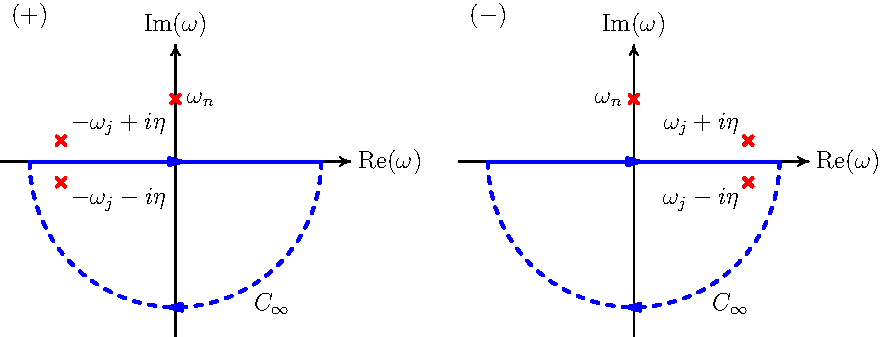
\includegraphics{contour.pdf}
\caption{Contours for integral $I_{\pm}$~\eqref{integral_I}. The $C_{\infty}$ arcs do not contribute thanks to Jordan's lemma.}
\label{contour}
\end{figure}
simplifying~\eqref{Pi_with_eta} to
% (which is consistent with~\eqref{exact_Pi_from_delta} for $\eta\rightarrow0$)
\begin{align}
\Pi(i\omega_n)
\approx
\sum_{j=i}^{J}
\frac{2a_j\omega_j}{\omega_j^2+(\omega_n+\eta)^2}.
\label{Pi_lorentz}
\end{align}

Therefore,~\eqref{sigma_lorentz} and~\eqref{Pi_lorentz} can be used to generate $p(\omega)$ and $\Pi(i\omega_n)$ data without having to perform costly numerical integrals. We can further get arbitrary $p(\omega)$ either by modulating the peak amplitudes $a_j$, or we can distribute their centers $\omega_j$ non-uniformly. The resulting function will be smooth as long as the width of the peaks are at least twice as large as the spacing between them, and the moments of the spectrum will be well-defined if a large enough number $J$ of Lorentzians are summed. Unfortunately, in practice, this sum can become as costly as a numerical integral.

\end{document}

